\chapter{Reaktivität auf der Anwendungsebene}
\label{chap:reaktivitaet_auf_der_anwendungsebene}
\section{Einführung}
Reaktivität auf der Anwendungsebene bedeutet die reaktive Programmierung einer Anwendung oder Teile einer Anwendung.
Per definitionem beschreibt die reaktive Programmierung einen Programmierstil, in dem ein Problem in Teilschritte zerlegt wird, wobei jeder Teilschritt eventbasiert, \glslink{Asynchronitaet}{asynchron} und nicht-blockierend verarbeitet werden kann. \footnote{vgl. Jog, S. 14 \cite{buch:reactive_programming_with_java9:kapitel1}}

Als Beispiel dient hier das Programm Excel. Hier ist eine Summenzelle definiert, die die Summe aus dem Inhalt einer Spalte berechnet. Wenn nun eine Zelle der Spalte sich in ihrem Wert ändert, wird ein Event angestoßen, sodass die Summenzelle die Summe neu berechnet. \footnote{vgl. Wikipedia, 2018 \cite{web:wiki:reactive_programming}}

Der Hauptgrund für die reaktive Programmierung ist, dass blockierendes Warten durch asynchrone Verarbeitung vermieden wird. Durch die Auslagerung der Operationen auf einen anderen Thread wird zum einen der Mainthread nicht blockiert, was zur Folge hat, dass die Anwendung nach wie vor bedienbar bleibt. Zum anderen können diese Threads auf Multikernprozessoren parallelisiert werden und die Gesamtauslastung somit optimieren. \footnote{vgl. Bonér und Klang, S. 6-8 \cite{technischer_bericht:lightbend:rpvsrs} \label{lightbend:rpvsrs}}

Konzepte, die die reaktive Programmierung umsetzen sind: Reactive Streams, Futures \& Promises und Dataflow-Variablen (beispielsweise Excel). \footref{lightbend:rpvsrs}

Die nachfolgenden Kapitel befassen sich mit der Umsetzung der reaktiven Programmierung sowie der Frage, wie sich die reaktive Programmierung von den reaktiven Systemen abgrenzt.

\section{Reactive Streams}
\label{sec:reactive_streams}
\subsection{Überblick}
Reactive Streams bezeichnen einen Standard für asynchrone Verarbeitung mit Back Pressure. Im Jahr 2013 entwickelten Mitarbeiter von u. a. Netflix, Lightbend und Pivotal diese Standardisierung. Die Standartisierung definiert Java Interfaces und bietet ein Technology Compatibility Kit zur Kompatibilitätsprüfung eigener Reactive Streams Implementierungen an.\footnote{vgl. Wikipedia, 2018, Reactive Streams \cite{web:wiki:reactive_streams}}

Die Reactive Streams entstanden aus dem Problem heraus, dass in asynchronen Anwendungen Daten stocken können. Dies passiert genau dann, wenn Daten schneller zur Verfügung stehen, als sie verarbeitet werden. Das wäre zum Beispiel der Fall, wenn Echtzeitdaten über einen Stream von einer langsamen Berechnung gestaut werden. Meist hat der verarbeitende Teil einen Puffer, um mit solchen Problemen umzugehen. Allerdings kann dieser Puffer überlaufen und somit einen Datenverlust verursachen. Um dieses Problem zu lösen, definiert die Reactive Streams Specification, wie Informationen mittels Back Pressure übertragen werden. Back Pressure ermöglicht eine regulierte Übertragung der Daten.\footnote{vgl. Reactive Streams, The Problem; Working Groups \cite{web:site:reative_stream_specification} \label{rss}}
Im Kapitel \ref{subsubsec:backpressure} wird Back Pressure ausführlicher behandelt.

Die definierten Java Interfaces müssen nach der Spezifikation implementiert werden, um Back Pressure zu ermöglichen. Die Spezifikation ist eine Sammlung von Regeln für Implementierer. Mit der Version 9 von Java wurden die Reactive Streams Interfaces ins eigene Repertoire aufgenommen und befinden sich im Modul java.base im Package \href{https://docs.oracle.com/javase/9/docs/api/java/util/concurrent/Flow.html}{java.util.concurrent}. Die Interfaces entsprechen exakt den Interfaces der Reactive Streams Specification. \footref{rss}
\clearpage
Prinzipiell besteht das Set aus vier Interfaces.
\begin{enumerate}
\item Ein Publisher, der den eigentlichen Stream definiert.
\item Ein Subscriber, der die Daten aus dem Stream empfängt.
\item Eine Subscription, die einen Subscriber einem Publisher zuordnet und den Datentransfer umsetzt.
\item Ein Processor, der die Eigenschaften eines Publishers und eines Subscribers in sich vereint.
\end{enumerate} 
\footnote{vgl. Github, Specification \cite{web:github:reactive_streams}}

Das folgende Sequenzdiagramm zeigt den Lebenszyklus eines Reactive Streams, wobei nur die Beziehung zwischen Publisher und Subscriber betrachtet wird.
\begin{figure}[H]
    \caption{Lebenszyklus eines Reactive Streams}
    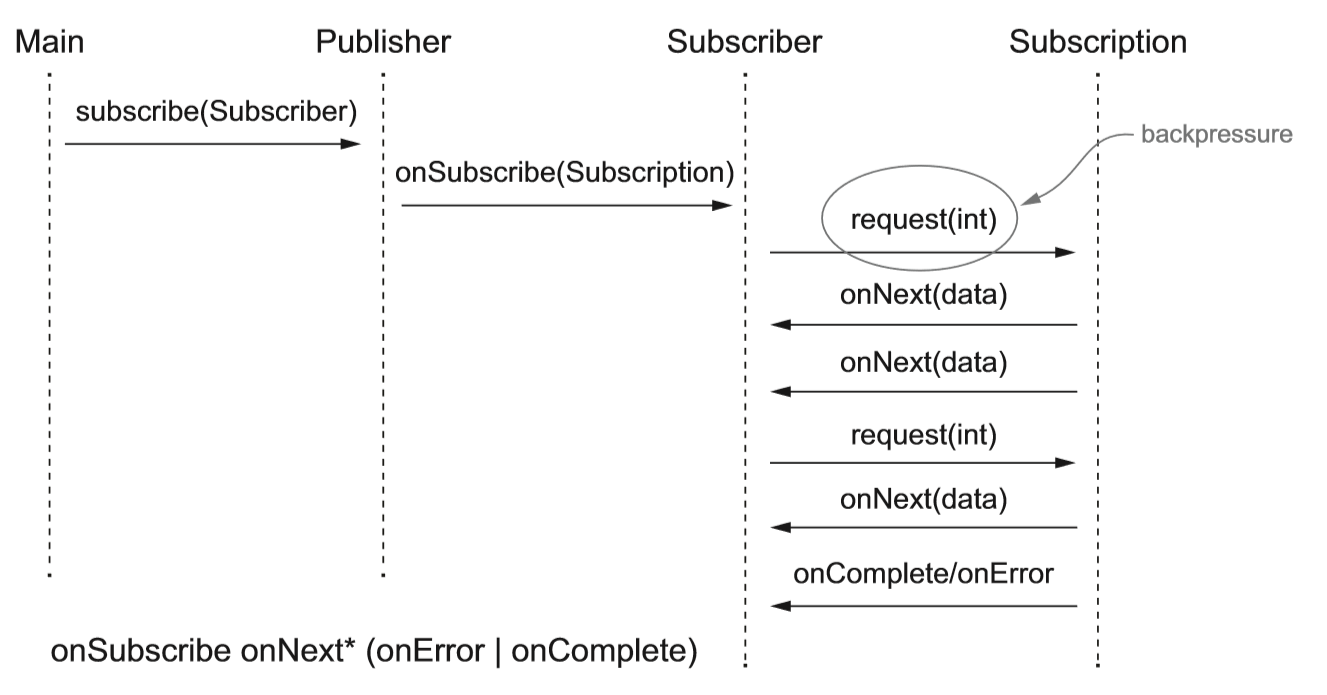
\includegraphics[width=\linewidth]{media/lifecycle}
    \label{lifecycle}
\end{figure} \footnote{vgl. Urma et al., S.424 \cite{buch:modern_java_in_action:kapitel17}}

Innerhalb des Mainthreads wird die Subscribe-Funktion, mit dem Subscriber als Argument, beim Publisher aufgerufen. Der Publisher ruft auf dem übergebenen Subscriber die Funktion onSubscribe auf, wobei die eine Subscription-Instanz des Publishers als Argument übergeben wird. Der Subscriber fordert eine bestimmte Anzahl an Datensätzen über die Request-Methode an. Die Subscription-Instanz ruft für die Anzahl an benötigten Daten die onNext-Methode des Subscribers auf. Dies geschieht, solange die Subscription keine onComplete- oder onError- Methode aufruft, denn damit ist die Subscription offiziell beendet. Die Request-Methode spielt hierbei eine besondere Rolle. Über diese lässt sich der Back-Pressure-Mechanismus realisieren, was im Kapitel \ref{subsubsec:backpressure} genauer betrachtet wird.

Anbieter wie z. B. RxJava, Reactor oder Akka implementieren die Reactive Streams Specifications.
So heißen die Reactive Streams in RxJava Flowable, in Akka-Streams Source und in Reactor Flux. Eine eingehendere Behandlung erfahren diese Begriffe in Kapitel \ref{chap:evaluierung}.
\subsection{Back Pressure}
\label{subsubsec:backpressure}
Unter Back Pressure versteht man die Regulierung des Datenflusses. In asynchronen Anwendungen kann es häufig zu einem Stau von Daten kommen, wenn beispielsweise der Publisher schneller Daten produziert als der Subscriber sie verarbeitet. Es gibt prinzipiell zwei Möglichkeiten, einen solchen Stau ohne Back Pressure zu vermeiden. \footnote{vgl. Grammes \& Schaal, 2015, S.44-45 \cite{web:artikel:javaspektrum} \label{grammesschaal}}
\begin{enumerate}
\item Der Subscriber reagiert auf den Stau und ordnet die Daten in eine Warteschlange ein. \footref{grammesschaal}
\item Der Publisher sendet kontinuierlich eine begrenzte Menge an Daten, sodass der Subscriber die Menge staufrei verarbeiten kann. \footref{grammesschaal}
\end{enumerate}

Bei Möglichkeit 1 kommen zwei Probleme auf. Wenn erstens die Größe der Warteschlange unbegrenzt ist, wird der Hauptspeicher irgendwann voll sein und einen Speicherüberlauf auslösen. Zweitens kann eine limitierte Größe der Warteschlange Datenverlust verursachen, wenn die Schlange voll ist.  \footref{grammesschaal}

Bei Möglichkeit 2 kann es passieren, dass die Leistung des Subscribers nicht vollständig ausgenutzt wird, wenn der Publisher zu wenig Daten produziert.  \footref{grammesschaal}

Back Pressure ermöglicht Überlastschutz über eine dynamische Anpassung des Datenflusses. Die Umsetzung gelingt über einen Push-Pull-Mechanismus. Push bezeichnet hier die Propagierung von Daten. Pull bezeichnet hingegen das Abholen von Daten. So wäre ein Push sinnvoll, wenn der Subscriber schneller als der Publisher ist, und ein Pull im gegenteiligen Fall.  \footref{grammesschaal}

Der Mechanismus des Back Pressure funktioniert so, dass zu Beginn davon ausgegangen wird, dass der Subscriber die Daten genauso schnell verarbeitet, wie der Publisher sie bereitstellt. Entsteht nun ein Stau, wechselt der Betrieb von Push zu Pull, was bedeutet, dass der Subscriber nun die Datenmenge anfordert, die er auch verarbeiten kann. So wird stets garantiert, dass zum einen kein Stau entsteht und zum anderen der Subscriber voll ausgelastet ist. \footref{grammesschaal}

\subsection{Streams oder Futures} \label{FutuProm}
Reactive Streams sind eine Spezifikation mit der Funktion, Informationen asynchron, nicht-blockierend und regulierend (Back Pressure) zu übertragen. Die Idee zur asynchronen, nicht-blockierenden Verarbeitung ist nicht neu und wurde bereits mit anderen Konzepten umgesetzt.

Futures sind Technologien die, wie Reactive Streams, reaktive Programmierung umsetzen.
Hierbei sind Futures ein Feature, das es bereits seit der Java-Version 5 gibt und im Package java.util.concurrent zu finden ist. Das Konzept dabei ist, eine Task asynchron durchzuführen, um blockierendes Warten zu vermeiden. Beim Aufruf wird direkt ein Future, also eine Referenz auf ein Ergebnis, geliefert, während die Task asynchron verarbeitet wird. Das Problem hierbei ist, dass einerseits der Status des Futures abgefragt werden muss, um zu erfahren, ob ein Ergebnis vorliegt. Andererseits kann es passieren, dass die asynchrone Task das Ergebnis nicht berechnet (Fehlerfall) und das Ergebnis somit nicht mehr verfügbar ist. Des Weiteren stellt es sich als schwer heraus, Ergebnisse von Futures aneinander zu reihen, da jedes Future wiederum auf Verfügbarkeit geprüft werden muss.\footnote{vgl. Urma et al., S.390 \cite{buch:modern_java_in_action:kapitel16} \label{futuresnpromisses}}

Seit der Java Version-8 wurden die CompletableFutures (java.util.concurrent), als konzeptuelle Erweiterung eingeführt. Die CompletableFutures können, im Gegensatz zu den Futures, verknüpft werden. Wenn eine asynchrone Operation von dem Ergebnis einer anderen abhängt, muss nun nicht-blockierend gewartet werden, bis das Ergebnis vorliegt, sondern kann direkt weitergeleitet werden. \footref{futuresnpromisses}

Sowohl Reactive Streams als auch Futures haben das Ziel, Tasks asynchron und nicht blockierend auszuführen. Der wesentliche Unterschied dieser Konzepte ist, dass Futures immer ein Element verarbeiten. So können zum Beispiel mehrere HTTP-Requests je in einem Future gemacht werden, während ein Stream keine theoretische Begrenzung hat. Des Weiteren sind Reactive Streams in der Lage, mittels Back Pressure Datenstaus zu vermeiden.

Die folgende Tabelle\footnote{vgl. Nurkiewicz und Christensen, Cardinality \cite{buch:reactive_programming_with_rxjava:kapitel1}} zeigt die Kardinalität von Technologien im asynchronen und synchronen Kontext: 

\begin{table}[H]
\centering
\caption{Szenarien und empfohlene Technologien}
\label{tab:scenariosandtech}
\begin{tabular}{
>{\columncolor[HTML]{C0C0C0}}l |c|c|}
\cline{2-3}
                                                        & \multicolumn{1}{l|}{\cellcolor[HTML]{00A99D}Ein Datensatz}                       & \multicolumn{1}{l|}{\cellcolor[HTML]{00A99D}Viele Datensätze}       \\ \hline
\multicolumn{1}{|l|}{\cellcolor[HTML]{00A99D}Synchron}  & Objekt                                                                           & \begin{tabular}[c]{@{}c@{}}Iterable,\\ Java Streams\end{tabular}    \\ \hline
\multicolumn{1}{|l|}{\cellcolor[HTML]{00A99D}Asynchron} & \begin{tabular}[c]{@{}c@{}}Callback, \\ Future,\\ CompletableFuture\end{tabular} & \begin{tabular}[c]{@{}c@{}}Reactive Stream,\\ Callback\end{tabular} \\ \hline
\end{tabular}
\end{table}

Für einfache synchrone Verarbeitungen mit einem Datensatz können simple Getter-Methoden genutzt werden, um das jeweilige Objekt zu erhalten. Falls viele Daten synchron verarbeitet werden müssen, eignen sich Iterable Typen respektive Streams. Im asynchronen Fall bieten sich Futures an. Selbst wenn es mehrere asynchrone Requests braucht, um eine Tasks zu verarbeiten, können dennoch CompleteableFutures verwendet werden. Bei vielen, asynchronen Datensätzen eignen sich vor allem die Reactive Streams.

\subsection{Collections API und Reactive Streams}
Der Begriff Stream kommt nicht nur in der reaktiven Programmierung vor, sondern auch in Java als native Bibliothek. Die Collections (in java.util.stream) unterstützen Streams als zusätzliche Abstraktionsebene, um deklarativ Informationen zu verarbeiten. Der so entstehende Vorteil ist, dass nun auf den imperativen Code von iterativen Schleifen verzichtet werden kann, was den Code allgemein wartbarer und verständlicher macht. Allerdings sind die Java Streams auf bestimmte Szenarien optimiert. Wie die Tabelle \ref{tab:scenariosandtech} zeigt, liegt die Stärke der Streams darin, Informationen synchron zu verarbeiten. Zwar ist es möglich, asynchrone Tasks zu verarbeiten, jedoch bietet die Streams-Api keine Möglichkeiten an die asynchronen Ergebnisse zu sortieren und zu synchronisieren. Vor allem in Situationen, in denen die asynchronen Tasks Latenzen haben oder undefinierte Zeitabstände vorweisen. Dies müsste manuell gelöst werden und würde die Komplexität des Codes stark erhöhen. Zudem gibt es keinen Mechanismus, der die Streams vor Überbelastung schützt.

Der Grund dafür, weshalb Java Streams in einen Kontext mit Reactive Streams gebracht werden, ist zum einen der Bezeichner Stream und zum anderen die deklarative Programmierung. Im späteren Teil dieser Thesis werden Implementierungen von Reactive Streams vorgestellt, die sich ähnlich deklarativ programmieren lassen wie die Java Streams. Die Möglichkeit der deklarativen Programmierung ist kein verpflichtendes Feature der Reactive Streams Specification und ist somit auch kein Teil von ihr.

Zusammengefasst liegt der Unterschied in dem Einsatzzweck: Java Streams sind für statische Daten geeignet, die einmal transformiert werden. Reactive Streams dagegen sind für dynamische, asynchrone Daten geeignet.

\subsection{Hot und Cold Streams}
\label{subsec:hotncold}
In vielen Implementierungen von Reactive Streams gibt es zwei Arten von Streams. Die Standard-Art ist der Cold Stream. Er reagiert mit dem Versenden der Daten, wenn eine Subscription erstellt wurde. Diese Art der Reaktion wird auch als lazy evaluation bezeichnet. Eine weitere Besonderheit ist, dass ein Cold Stream immer die gesamten Informationen für jede Subscription versendet. Ein Cold Stream ist somit nicht für Echtzeitdaten geeignet. Dieser Stream-Typ eignet sich besonders dann, wenn Informationen ein definiertes Ende haben, wie z. B. beim Inhalt einer Textdatei. \footnote{vgl. Davis, Hot and Cold \cite{buch:reactive_streams_in_java:kapitel3} \label{hot_and_cold}}

Ein Hot Stream dagegen versendet Daten unabhängig von Subscriptions. Das heißt, dass ein Subscriber immer die aktuellen Daten des Streams anstelle des gesamten Datensatzes empfängt. Hot Streams eignen sich dann, wenn die Informationen kein definiertes Ende haben, wie z. B. bei Twitter-Feeds. \footref{hot_and_cold}

\section{Reaktive Programmierung in reaktiven Systemen}
\label{sec:rpinrs}
Ein reaktives System ist ein Modell, das anhand von Qualitäten ein modernes, antwortbereites System beschreibt. Die reaktive Programmierung ist ein Paradigma, das Datenstrukturen in Streams asynchron, und nicht-blockierend verarbeitet. Beide Kontexte lassen sich miteinander vereinen, jedoch eignen sich die meisten reaktiven Bibliotheken nicht dafür, reaktive Systeme zu bauen.

Der Grund dafür ist die eventbasierte Kommunikation. Events haben keinen klaren Empfänger und stellen lediglich Fakten oder Signale dar. Die Widerstandsfähigkeit und Elastizität sind nicht ohne Weiteres realisierbar, da eine nachrichtenorientierte Kommunikation notwendig ist (siehe Kapitel \ref{sec:das_reaktive_manfiest}). Ein isolierter, ausgefallener Service muss adressierbar sein; falls er das nicht ist, weiß das System nicht, welcher Service wiederhergestellt werden soll.

Reaktive Programmiertechniken sind auf zeitlicher Ebene gut skalierbar, das heißt, sie sind für Nebenläufigkeit optimiert, während reaktive Systeme auf örtlicher Ebene skalierbar und daher verteilbar sind. Um ein reaktives System aus reaktiven Programmiertechnologien wie Streams und Futures zu bauen, benötigt es somit ergänzende Technologien wie z. B. Nachrichtenbusse, Fehlererkennungstechnologien (bspw. Hystrix) und Replikationstechniken (bspw. Docker).
\footnote{vgl. Benedikt Stemmildt \cite{web:youtube:going_reactive}; Bonér und Klang, S. 15 \cite{technischer_bericht:lightbend:rpvsrs}}

Ein prominentes Beispiel für die Verwendung von reaktiver Programmierung in reaktiven Systemen ist das Akka Toolkit. Die interne Verarbeitung der Daten und die Weiterleitung an Operatoren wird über eine Reactive-Streams-Implementierung realisiert. Das \href{https://akka.io/docs/}{Akka Toolkit} enthält noch weitere Technologien wie z. B. eine Implementierung des Aktorenmodells über die sich Nachrichten zwischen verschiedenen Diensten austauschen lassen. Es ist möglich, vollständige reaktive Systeme mit dem Toolkit zu bauen, da notwendige Technologien für die Streams bereits integriert sind. Anders als bei reinen Streams-Implementierungen wie RxJava und Reactor werden somit keine externen Abhängigkeiten (wie z. B. Message Bus und Verteilungssoftware) benötigt, was die \glslink{Homogen}{Homogenität} des gesamten Systems erhöht.

Es bietet sich an, die Dienste eines reaktiven Systems mit reaktiven Programmiertechniken zu bauen, denn auf der Anwendungsebene ist die reaktive Programmierung eine Alternative zu synchronen und blockierenden Programmen. In Kapitel \ref{chap:umsetzung} wird eine Anwendung reaktiv und klassisch implementiert, was im Anschluss in Performancetests miteinander verglichen wird.   